\documentclass{LTHthesis}
\usepackage[T1]{fontenc}
\usepackage[utf8]{inputenc}  %% Comment if you are not using utf8
\usepackage{mathptmx, helvet}
%\usepackage[swedish]{babel}  %% aktivera om rapporten är på svenska
\usepackage{amsmath}
\usepackage{amsfonts}
\usepackage{amssymb}

\usepackage{graphicx}

\addbibresource{mybib.bib}  %%  Comment if you don't want to use bibtex.

\begin{document}
\begin{titlepages}
\author{Martin Djup and Elias Allar}
\title{Sensorless Control of BLDC\\ in Hydraulic Application}
\year{2015}
\month{June}
\TFRT{9999}  %%  You will get the number from the department.
\printer{Media-Tryck}  %% Probably. You may get other information from the department.
\end{titlepages}
\chapter*{Abstract}
A condensed description of my work.
\chapter*{Acknowledgements}
These people helped me a lot with my work.
\tableofcontents
%NOMENCLATURE? ABBREVIATIONS MM.?

%\chapter{Introduction}
%\section{Organization}
%First of all, the theory and fundamentals behind the BLDC and control methods needs to be understood if one is to understand the results of this thesis. In chapter 2 the most central theory and fundamentals used in this thesis is collected.
%KOLLA SÅ RÄTT KAPITEL!!!
%
%In order to study if a sensorless BLDC is feasible to control the pump according to specifications, the BLDC and control methods were first built in Simulink. The implementation in Simulink is described in chapter 3. 
%KOLLA SÅ RÄTT KAPITEL!!!
%
%Since the possibility of changing the currently used DC motor to a sensorless BLDC was of great interest to BW TTS, the control methods were also tested on real hydraulic pumps after the Simulink results had been analyzed. Also, an evaluation of cost and computational feasability of the controller were tested. This is all described in chapter 4.
%KOLLA SÅ RÄTT KAPITEL!!! TA BORT DET SISTA OM VI INTE HINNER MED DET.
%
%The goal of the thesis was to be able to draw conclusions on possibilities of using a sensorless BLDC in the hydraulic application based on simulations and testing. Several conclusions could be drawn, and are discussed in chapter 5.
%KOLLA SÅ RÄTT KAPITEL!!!


%A Simulink model of the hydraulic pump was provided by BW TTS which was used to test the BLDC and the control methods. The pump model was important in order to be able to give the right torque load on the BLDC model.
%
%In order to get good control of the BLDC the sample time was chosen to be fairly fast. It has the value $T_{s}=0.0001$s.

\chapter{Introduction}
asdfc
%This is a description of my work. 

This thesis was conducted by two students from the faculty of engineering at Lund University and was made in corporation with BorgWarner TorqTransfer Systems AB (BW TTS for short) in Landskrona, Sweden. The main purpose of the thesis was to study the possibilities of implementing sensorless control techniques for a BLDC (Brushless Direct Current Motor) used in a hydraulic application. By sensorless, the meaning is that the position and speed of the rotor on the BLDC is unknown to the controller and has to be estimated in some way.
There are many ways of controlling a sensorless BLDC which may all lead to different results on aspects such as torque ripple and required computational power. Mainly two control techniques were studied and tested in this thesis. The first, which most focus was laid on was the FOC (Field-Oriented Control) with field weakening. The second was six-step commutation which is a little bit simpler in nature than the FOC. Both control methods were chosen since they can work well with sensorless methods.
%The hydraulic application that is to be controlled is a pump, and the BLDC has to be fast and strong enough to the able to handle certain specifications, i.e. being able to rotate at certain speeds while handling corresponding torque load from the pump. 
\section{Background}
BorgWarner TorqTransfer Systems AB focuses on AWD-Systems (All-Wheel Drive Systems) for the car industry and it centers around a certain clutch which is able to distribute the driving torque on the wheels when necessary. This clutch is used by several car manufacturers and is in constant development. The torque distribution is driven by a hydraulic pump which obtains its pressure from rotation of the driving axle of the car, and is then controlled by a small electrical motor. Today, the electrical motor used in the hydraulic application is a simple DC motor. It has proven to be fairly easy to control and implement, but the life time of the motor does not always live up to the expectations of the clutch. Since said clutch is directly linked to the driving performance of the car, the response time and performance of the motor  controlling the hydraulic pressure is critical. There must also not be too much ripple in the provided torque and speed from the motor in order to get good performance from the clutch.
\section{Motivation}
The car industry in general is a very hard and pressured industry, so all components has to be as cheap as possible and yet robust so that they may survive the life cycle of the whole vehicle. BW TTS has in later years been looking at other means of controlling the hydraulic pressure than the standard DC motor since this is one of the main components that seem to fail when there is a problem with the clutch. One of the reasons that the DC motor fails is that it is a brushed motor, i.e. it uses a commutator. When the commutator is brushed against the rotor it is exposed to a lot of wear and may need maintenance more often than other components \cite{ala_kar2014}. In a brushless motor on the other hand, the number of moving parts are limited to the rotor, and due to this fact brushless motors has grown on the market in recent years.
From this, one can see that a brushless motor would be a better choice for the hydraulic application in mind, even though controlling it is a little bit more difficult. That is the reason for why the possibility to use a BLDC was studied in this thesis. 
However, an ordinary BLDC assumes that the rotor angle and speed is always known to the control unit of the motor. This is often realized by using sensors to detect the position of the rotor. Since sensors are both costly and makes the application less reliable, a sensorless control is the only feasible alternative in this type of clutch for the car industry.

\section{Organization}
In order to study if a sensorless BLDC is a feasible alternative to control the hydraulic pump according to specifications, the BLDC and control methods were first built in Simulink. The Simulink implementation of the BLDC and control schemes was the main part of this thesis, and therefore most of the work was put here. In order to build the entire sensorless control of the BLDC in Simulink it was important to test it continuously during the construction so that it would all work well in the end. It was made in the following steps:
\begin{enumerate}
\item Construct a working BLDC model
\item Implement FOC with known rotor angle, i.e. non-sensorless control
\item Make the FOC sensorless
\item Implement six-step commutation
\item Evaluate Simulink results
\end{enumerate}
These steps, together with necessary theoretical backgrounds, are described in the first chapters of this thesis. Chapter 2 describes the fundamentals behind the BLDC and how it was constructed in Simulink.
Chapter 3 describes how the non-sensorless FOC controller was implemented in Simulink, together with theoretical motivations.
Chapter 4 is a theoretical chapter which describes methods for making the control sensorless. It also shows how sensorless control was implemented in this thesis.
After the implementation of sensorless FOC was complete, the sensorless six-step commutation method was also implemented in Simulink. It was made so that it could be compared to the sensorless FOC. The sensorless six-step commutation implementation is described in chapter 5.

With the implementation of both sensorless FOC with field weakening and sensorless six-step commutation complete, the results of the Simulink implementations were evaluated. This is done in chapter 6.

Since the possibility of changing the currently used DC motor to a sensorless BLDC was of great interest to BW TTS, the control methods were also tested on real hydraulic pumps after the Simulink results had been analyzed. Also, an evaluation of cost and computational feasibility of the controller were tested. This is all described in chapter 7.

The goal of the thesis was to be able to draw conclusions on possibilities of using a sensorless BLDC in the hydraulic application based on simulations and testing. Several conclusions could be drawn, and are discussed in chapter 8.
RÄTT KAPITEL ÖVERALLT???


\chapter{The Brushless DC Motor}
As the name implies, the BLDC differs from an ordinary DC motor in the way that it lacks a brushed commutator. However, this is not the only way that it differs. 
While an ordinary DC motor has its permanent magnets on the stator, the BLDC has its permanent magnets located on the rotor. On the stator of the BLDC there are coils divided into three pairs (one for each phase). This might sound to some as what they know as a PMSM (Permanent Magnet Synchronous Motor), and they can be considered being one and the same. If one were to study literature and articles published in this area one will find that there is no clear standard of what counts as a BLDC and what counts as a PMSM. Some suggest that the motor is a PMSM if it uses sinusoidal commutation while it is a BLDC when it uses trapezoidal commutation \cite{lee_lem_keo}. The way of commutation comes directly from the control method, e.g. FOC gives sinusoidal commutation and six-step gives trapezoidal commutation. Very simplified, one can say that the commutation method tells what form the input voltage have on the three phases on the motor. 
%commutations sinus vs trap. ELLER är det bara FOC vs Six step? <-svarat på?

\section{Vector Reference Frames}
When working with control of synchronous electrical drives, mainly three vector reference frames are used. The first two are in the stator frame, and the last one is in the rotor frame. All three can be seen in figure \ref{ref_frames}
\begin{figure}
\centering
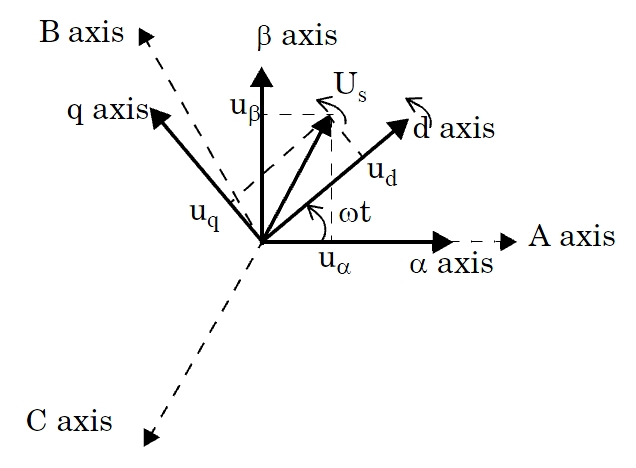
\includegraphics[width=8cm]{ref_frames_mathworks}
\caption{Stator voltage $U_{s}$ and its respective components in the three reference frames, \cite{ref_frames}.}
\label{ref_frames}
\end{figure}
\subsection{a/b/c-frame}
The first reference frame is called the a/b/c-frame and it uses three vector components, each in the same two dimensions but with 120 degrees between each other. This reference frame is pedagogic to work with since the motor is driven by a three-phase source, and each of the three vector components are aligned with each stator coil pair. In this frame one can easily witness the magnitude of currents and voltage in each phase and is very good for practical reasons. The three phases are the only inputs to the motor, and it is only in said phases that the behavior of a sensorless motor is observable. E.g. for any given input voltage, there will run a current in the motor from which conclusions can be drawn about the behavior of the motor. This is later used when making the control sensorless.
\subsection{$\alpha/\beta$-frame}
Working with three vectors in two dimensions seems unnecessary when the placement of the coils is of no interest. So when only the vectors themselves are of interest, without relation to the phases or the stator coils, one can use the Clarke transformation in order to transform the a/b/c-frame to the $\alpha/\beta$-frame, see \eqref{clarke}.
\begin{subequations} \label{clarke}
\begin{align} 
s_{\alpha}&=\sqrt{\frac{3}{2}}s_{a}\\
s_{\beta}&=\sqrt{\frac{1}{2}}(s_{b}-s_{c})
\end{align}
\end{subequations}
The $\alpha/\beta$-frame is also a stator frame but with the $\alpha$-component aligned to the a-component and the $\beta$-component orthogonal to the $\alpha$-component. So the $\alpha/\beta$-frame is similar to the typical x- and y-axes of a 2-dimensional system, but centered on the stator of an electrical motor. It is of course possible to make an inverse Clarke transformation in order to go from $\alpha/\beta$-frame to the a/b/c-frame, see \eqref{invclarke}.
\begin{subequations} \label{invclarke}
\begin{align}
s_{a}&=\sqrt{\frac{2}{3}}s_{\alpha}\\
s_{b}&=-\sqrt{\frac{1}{6}}s_{\alpha}+\sqrt{\frac{1}{2}}s_{\beta}\\
s_{c}&=-\sqrt{\frac{1}{6}}s_{\alpha}-\sqrt{\frac{1}{2}}s_{\beta}
\end{align}
\end{subequations}
One should note that the Clarke- and inverse Clarke transformations presented here are the so called power invariant transformations, but there is at least one other possible way to do the transformations called the amplitude invariant transformations. The amplitude invariant transformations are however more suitable for example in audio applications, where preserving the amplitude may be of great importance \cite{ala_kar2014}.
\subsection{d/q-frame}
The final reference frame is similar to the $\alpha/\beta$-frame, but is fixed on the rotor instead of the stator. This practically means that the d/q-frame is the same as the $\alpha/\beta$-frame with the difference being that the d/q-frame is rotated by the rotor angle. This means for example that when the rotor angle is zero, the two reference frames are the same. The d/q-frame is very useful for then looking at vectors form the rotor's point of view, and it can sometimes also be called the x/y-frame. Only in asynchronous motors are the d/q- and x/y-frame different. Going from a/b/c-frame to the d/q-frame is called the Park transform. And similarly, going from d/q-frame to the a/b/c-frame is called the inverse Park transform. For simplicity, one can instead look at the transformations between $\alpha/\beta$-frame and d/q-frame (which are the same but with negative rotor angle $\omega t$ inserted in $\alpha/\beta$- to d/q-frame transformation). See \eqref{dqalphabeta}.
\begin{subequations} \label{dqalphabeta}
\begin{align} 
s_{d/\alpha}&=s_{\alpha/d}cos(\omega t)-s_{\beta/q}sin(\omega t)\\
s_{q/\beta}&=s_{\alpha/d}cos(\omega t)+s_{\beta/q}sin(\omega t)
\end{align}
\end{subequations}

\section{Fundamentals of the BLDC}
A BLDC can be viewed as in figure BILD PÅ 11.2 FRÅN MATS BOK. The three inductance symbols outside of the stator are representations of the inductances of the three coil pairs from the three input phases. One might just imagine that the coils have been "pulled off" from the stator and put right outside. 

The main task of an electrical drive such as the BLDC is to produce torque, which makes the rotor spin. The torque is produced by making the theree-phase inputs produce a voltage vector in a certain direction and then let this vector rotate around its center point. This voltage vector produces a magnetic flux vector due to the input coils that the three-phase inputs are connected to. Since this magnetic flux vector comes from the stator, which cannot rotate, the flux of the permanent magnets on the rotor will want to align itself to the stator flux vector. So by letting the rotor flux vector "chase" the stator flux vector, torque and speed is produced.

The rotor in figure SAMMA SOM OVAN seems to have only one pole pair on its permanent magnets, but on the BLDCs that are to be used in the hydraulic application have magnetic poles equally spaced around the rotor. However, it is still possible to model the rotor as in figure BILD 11.2 FÅRN MATS IGEN where the main magnetic flux from the permanent magnets that are linking to the stator windings, $\Psi_m$, is aligned to the d-axis of the rotor (x-axis in the figure). KOLLA IFALL DET ÄR X ELLER D.

The voltage vector in the BLDC can be expressed as a resistive voltage drop plus the derivative of the magnetic flux vector $\psi_s$, where the latter follows from Faraday's law of induction. In $\alpha/\beta$-frame this voltage vector can be rewritten as in \eqref{BLDC_voltageab}, \cite{ala_kar2014}.
\begin{equation} \label{BLDC_voltageab}
\vec{u}_s^{\alpha\beta}=R_s\vec{i}_s^{\alpha\beta}+\frac{d\vec{\psi}_s^{\alpha\beta}}{dt}=R_s\vec{i}_s^{\alpha\beta}+\frac{d}{dt}\big(\vec{\psi}_\delta^{\alpha\beta}+L_{s\lambda}\vec{i}_s^{\alpha\beta}\big)
\end{equation}
As seen in \eqref{BLDC_voltageab} the $\psi_s$-vector is expressed in the air gap flux $\psi_\delta$ and the stator leakage inductance times the stator current: $L_{s\lambda}i_s$. The air gap flux is the magnetic flux from the stator windings which reaches the rotor and is therefore the useful part. The other part of $\psi_s$ is the leakage flux $\psi_\lambda=L_{s\lambda}i_s$, which is the flux from the stator windings that does not reach the rotor. This makes the leakage flux not very useful for torque production in the motor. $L_\lambda$ can thus be seen as the part of the stator inductance which only contributes to leakage flux. The leakage flux is assumed to have the same magnitude in all directions in the $\alpha/\beta$-frame. If the rotational electric speed $\omega_{el}$ is known and if $j$ is the imaginary unit, \eqref{BLDC_voltageab} can be expressed in the d/q-frame. This is seen in \eqref{BLDC_voltagedq}.
\begin{equation} \label{BLDC_voltagedq}
\vec{u}_s^{dq}=R_s\vec{i}_s^{dq}+\frac{d}{dt}\big(\vec{\psi}_\delta^{dq}+L_{s\lambda}\vec{i}_s^{dq}\big)+j\omega_{el}\big(\vec{\psi}_\delta^{dq}+L_{s\lambda}\vec{i}_s^{dq}\big)
\end{equation}
If also the main inductances (the parts of $L_s$ which are not leakage inductances) in the d- and q-axis, $L_{md}$ and $L_{mq}$, are introduced \eqref{BLDC_voltagedq} can be written in its q- and q-components. The components are seen in \eqref{BLDC_voltagedandq}, \cite{ala_kar2014}.
\begin{subequations} \label{BLDC_voltagedandq}
\begin{align}
\nonumber u_{sd}&=R_si_{sd}+\frac{d}{dt}\big(\Psi_m+L_{md}i_{sd}+L_{s\lambda}i_{sd}\big)-\omega_{el}(L_{mq}i_{sq}+L_{s\lambda}i_{sq})=\\&=R_si_{sd}+\frac{d}{dt}\big(\Psi_m+L_{sd}i_{sd}\big)-\omega_{el}L_{sq}i_{sq}\\
\nonumber u_{sq}&=R_si_{sq}+\frac{d}{dt}\big(L_{mq}i_{sq}+L_{s\lambda}i_{sq}\big)+\omega_{el}(\Psi_m+L_{md}i_{sd}+L_{s\lambda}i_{sd})=\\&=R_si_{sq}+L_{sq}\frac{di_{sq}}{dt}+\omega_{el}(\Psi_m+L_{sd}i_{sd})
\end{align}
\end{subequations}
From \eqref{BLDC_voltagedandq} it is possible to find expressions for the magnetic fluxes in the d- and q-axis, see \eqref{BLDC_fluxes}, \cite{ala_kar2014}.
\begin{subequations} \label{BLDC_fluxes}
\begin{align}
\psi_{sd}&=\Psi_m+L_{sd}i_{sd}=\Psi_m+(L_{md}+L_{s\lambda})i_{sd}\label{BLDC_fluxes1}\\
\psi_{sq}&=L_{sq}i_{sq}=(L_{mq}+L_{s\lambda})i_{sq}\label{BLDC_fluxes2}
\end{align}
\end{subequations}
\subsection{Mechanical Quantities}
With the equations and vector orientations of magnetic fluxes, currents and voltages derived it is possible to look at the mechanical quantities such as torque, speed and rotor angle.
The first quantity to look at is the electric torque. It comes directly from the cross product of the magnetic fluxes and the stator current. This gives \eqref{BLDC_torqueel}, \cite{ala_kar2014}.
\begin{align} \label{BLDC_torqueel}
T_{el}&=\vec{\psi}_s\times\vec{i}_s=\psi_{sd}i_{sq}-\psi_{sq}i_{sd}=\nonumber\\&=(\Psi_m+(L_{md}+L_{s\lambda})i_{sd})i_{sq}-(L_{mq}+L_{s\lambda})i_{sq}i_{sd}=\nonumber\\&=\Psi_mi_{sq}+\underbrace{(L_{md}-L_{mq})i_{sd}i_{sq}}_\text{Reluctance torque}
\end{align}
As seen in \eqref{BLDC_torqueel} there are two components that produce the torque. The component marked as reluctance torque is called so because it depends on the difference in reluctance in the d- and q-axis, \cite{ala_kar2014}.

The electro dynamical torque, $T_{el}$, in \eqref{BLDC_torqueel} is not the mechanical torque one would feel while holding on to the rotor of a running motor. The electrical torque is the torque produced if there are only one magnetic pole pair, $p/2$, on the rotor. In order to get the mechanical torque, the electro dynamical torque has to be scaled by a factor which is the number of pole pairs, see \eqref{BLDC_torquemech}.
\begin{equation} \label{BLDC_torquemech}
T_{mech}=\frac{p}{2}T_{el}
\end{equation}
When the electro dynamical and mechanical torques are known, the mechanical speed is of interest. It is derived by integrating the mechanical torque and compensating for moment of inertia $J$, see \eqref{BLDC_speedmech}
\begin{equation} \label{BLDC_speedmech}
\omega_{mech}=\frac{1}{J}\int T_{mech}
\end{equation}
Just like the torque, the speed has to be compensated by the number of magnetic pole pairs if one wishes to transform the mechanical speed to electrical speed. By electrical speed, the meaning is how fast the period time of the electrically induced voltage is. The electrical speed is needed for calculation of the back emf, which is discussed below, so the equation for the electrical speed is presented in \eqref{BLDC_speedel}. ÄR EMF:N NÄMND SENARE ELLER FÖRE???
\begin{equation} \label{BLDC_speedel}
\omega_{el}=\frac{p}{2}\omega_{mech}
\end{equation}
If one considers the instantaneous power of the BLDC, the motivations behind \eqref{BLDC_torquemech} and \eqref{BLDC_speedel} can be motivated further. The instantaneous power must be the same in electrical quantities as in mechanical quantities, which is seen in \eqref{BLDC_instpower}.
\begin{equation} \label{BLDC_instpower}
p(t)=\omega_{el}T_{el}=\frac{p}{2}\omega_{mech}\frac{2}{p}T_{mech}=\omega_{mech}T_{mech}
\end{equation}
The final mechanical quantity that needs to be derived is the rotor angle. If e.g. the electrical speed is known, one only has to integrate it in order to get the electrical rotor angle, \eqref{BLDC_angleel}. The electrical angle $\theta_{el}$ is needed for e.g. Park transformations throughout the control unit. 
\begin{equation} \label{BLDC_angleel}
\theta_{el}=\int \omega_{el}
\end{equation}
Of course, the mechanical rotor angle can also be of interest, and just as for speed and torque it is obtained by scaling the electrical angle by the pole pairs, see \eqref{BLDC_anglemech}.
\begin{equation} \label{BLDC_anglemech}
\theta_{mech}=\frac{1}{p/2}\theta_{el}=\frac{2}{p}\theta_{el}
\end{equation}
Since this thesis focuses on control of an electrical drive, there is one more important thing to remember. That is, that the torque of the motor is proportional to the motor current, and that the speed in the same way is proportional to the voltage over it, \cite{ala_kar2014}. The relation between torque and current can be observed in \eqref{BLDC_torqueel}, and it is good to keep this relationship in mind when controlling an electrical drive since there might be a maximum allowed current in the motor which puts a limit on the produced torque.

\subsection{Electromotive Force}
The three-phase input of the BLDC is connected to coils that are supposed to give uprise to a magnetic flux. In order to make the rotor turn, the magnetic flux from the coils will have to change very often. Each of the coils will feel these rapid changes in fluxes and will try to preserve equilibrium by inducing a voltage in the opposite directions of the input voltages, all according to Lenz's law. If one now keeps in mind that the speed of the BLDC is proportional to the voltage, there will be more and more induced voltage in the opposite direction as the speed increases. The induced voltage is often called back emf (electromotive force) since it counteracts the speed which the BLDC is trying to build up.

One may take the thought of back emf one step further and imagine what would happen if the BLDC would try to increase its speed to infinity. Due to the back emf the speed of the BLDC will come to a point where the induced voltage is just as big as the input voltages. This will mean that there will be no net voltage over the BLDC inputs and therefore also no current. This will of course make the BLDC stop increasing its speed and settle at the speed it had when the back emf obtained the same value as the input voltages. This maximum reachable speed may prove a problem to electrical drives which are to run at high speeds, but there are ways of going around the problem of induced back emf. One such way is called field weakening, and is discussed together with FOC in the chapter 3. KOLLA SÅ RÄTT KAPITEL!!!

While working in the d/q-frame, the back emf can be presented as a vector which lies 90 degrees advanced forward compared to the stator flux vector $\psi_s$, \cite{ala_kar2014}. This means that the induced back emf can be written as \eqref{BLDC_emfvect}.
\begin{equation} \label{BLDC_emfvect}
\vec{e}_s=j\omega\vec{\psi}_s
\end{equation}
It is also possible to rewrite \eqref{BLDC_emfvect} in its d- and q-components while also exploiting the fact that the back emf is depending on the electrical speed of the BLDC. This is seen in \eqref{BLDC_emfdq}, \cite{ala_kar2014}.
\begin{subequations} \label{BLDC_emfdq}
\begin{align} 
e_{sd}&=-\omega_{el}\psi_{sq}=-\omega_{el}L_{sq}i_{sq}\\
e_{sq}&=\omega_{el}\psi_{sd}=\omega_{el}(\Psi_m+L_{sd}i_{sd})
\end{align}
\end{subequations}

\subsection{The BLDC as an RLE-Load}
With the concept of back emf and the other fundamentals in mind there is one more useful thing to observe about the BLDC which will be used later in parts of the FOC controller. That is to compare the BLDC to a generic three-phase load. A way to do this is seen in figure \ref{BLDC_rle}.
\begin{figure}
\centering
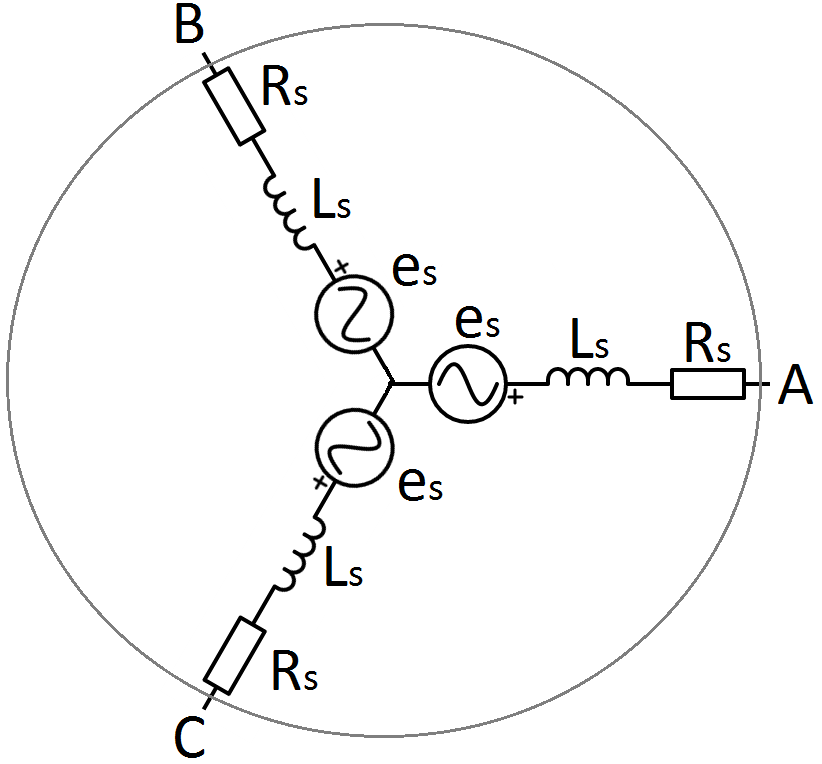
\includegraphics[width=8cm]{rle}
\caption{BLDC modeled as a generic three-phase load with phase resistance $R_s$, phase inductance $L_s$ and load voltage $e_s$.}
\label{BLDC_rle}
\end{figure}

The BLDC can as most electrical motors be viewed as a three-phase RLE-load with resistance $R_{s}$, inductance $L_{s}$ and load voltage $e_{s}$ on each phase (the load voltage being the back emf in an electrical drive). This means that the phase voltage of the BLDC can be written as \eqref{BLDC_RLEphasevoltage}.
\begin{equation} \label{BLDC_RLEphasevoltage}
u_{s}=R_{s}i_{s}+L_{s}\frac{di_{s}}{dt}+e_{s}
\end{equation}
This view can be motivated by combining \eqref{BLDC_emfdq} and \eqref{BLDC_voltagedandq}. The result is seen in \eqref{BLDC_RLEdq} and even though \eqref{BLDC_RLEdq} is written in the d- and q-components the similarity to \eqref{BLDC_RLEphasevoltage} is very notable.
\begin{subequations} \label{BLDC_RLEdq}
\begin{align}
u_{sd}&=R_si_{sd}+L_{sd}\frac{di_{sd}}{dt}+e_{sd}+\underbrace{\frac{d\psi_m}{dt}}_{\substack{\text{=0}\\\text{$\big(\Psi_m$ constant$\big)$}}}\\
u_{sq}&=R_si_{sq}+L_{sq}\frac{di_{sq}}{dt}+e_{sq}
\end{align}
\end{subequations}

\section{The BLDC Model in Simulink}
The finished BLDC model can be seen in figure FIGUR PÅ BLDC SIMULINKMODELLEN

The three phases enters as inputs va, vb, and vc. At first they are centered around zero in the Centering-block, which is done because the motor is galvanically isolated from the control unit, so there should be no eventual DC offset. After centering, the three phase voltages are transformed into the d/q-frame. 

By looking at the voltages in \eqref{BLDC_voltagedandq} and noticing that it with the help of \eqref{BLDC_fluxes} and \eqref{BLDC_emfdq} can be rewritten as \eqref{BLDC_voltagedandqREW}, it can be seen that the left hand sides of \eqref{BLDC_voltagedandqREW} is what comes out from the sum-block right after the transformation to d/q-frame.
\begin{subequations} \label{BLDC_voltagedandqREW}
\begin{align}
\frac{d\psi_{sd}}{dt}&=u_{sd}-R_si_{sd}-e_{sd}\\
\frac{d\psi_{sq}}{dt}&=u_{sq}-R_si_{sq}-e_{sq}
\end{align}
\end{subequations}
After \eqref{BLDC_voltagedandqREW} is applied, there is an integration which gives the fluxes $\psi_{sd}$ and $\psi_{sq}$. The fluxes are then saturated as not to produce values larger than twice that of $\Psi_m$, which is impossible. After that the fluxes in d- and q-axis are treated separately.

The current in d/q-frame is obtained by applying \eqref{BLDC_currentdq} which is given by rewriting \eqref{BLDC_fluxes}.
\begin{subequations} \label{BLDC_currentdq}
\begin{align}
i_{sd}&=\frac{\psi_{sd}-\Psi_m}{L_{sd}}\\
i_{sq}&=\frac{\psi_{sq}}{L_{sq}}
\end{align}
\end{subequations}
With the current at hand, the resistive voltage drop in \eqref{BLDC_voltagedandqREW} is modeled by a feed back with a gain corresponding to the resistance $R_s$.

The current in d/q-frame can be transformed into a/b/c-frame, which is done before the current is going out of the BLDC model in an output.

When all currents, voltages and fluxes are implemented in the model it is possible to implement the mechanics of the BLDC in the model.

First, the electrical torque is given by the first line of \eqref{BLDC_torqueel} and is then scaled by the number of pole pairs according to \eqref{BLDC_torquemech}. With the mechanical torque at hand it is possible to subtract the torque load which enters the BLDC model as an input.

After the torque load is accounted for equations \eqref{BLDC_speedmech}, \eqref{BLDC_speedel},\eqref{BLDC_angleel} and \eqref{BLDC_anglemech} are used to calculate the electrical and mechanical speeds and angles of the BLDC. All of these mechanics (except the electrical speed) then leaves the BLDC model as outputs so that they can be observed more clearly from the outside while testing the model ÄR OUTPUTS ENS KVAR???. The electrical angle is also fed back to the transformations from and to the d/q-frame. 

Finally, the back emf is calculated in the d/q-frame. This is where the electrical speed is used, all according to \eqref{BLDC_emfdq}. The back emf is then leaving the BLDC model as an output but is also used in the previous calculations \eqref{BLDC_voltagedandqREW}.

This concludes the most major part of the BLDC model constuction in Simulink. All that is left to do is to determine the BLDC parameters. 

\subsection{BLDC Model Parameters}
The BLDC model does not only depend on the known equations that are presented above. It also depends on certain parameters that are related to the real BLDC. There are a total of six parameters in the model that has to be chosen in order to make the model agree with a real BLDC. Most of these parameters could be obtained by looking at the BLDC specifications of the BLDC manufacturers that had given their specifications to BW TTS.

All of the BLDCs that were specified by the different manufacturers could handle the requirements for the hydraulic application, so the BLDC model made in Simulink should also be able to handle the requirements by using the parameters from any of the manufacturers. Since none of the them did  provide all of the required parameters in their specifications, the BLDC parameters from the manufacturer that provided most of them were chosen. The rest were either calculated or estimated.

Maybe the most central parameter is the number of magnetic poles on the rotor,  $p$. From the chosen manufacturer this was set to $p=10$.

The next parameter that was needed was the stator resistance, $R_{s}$. Since only the phase-to-phase resistance, $R_{p2p}$, was provided, and that this certain BLDC was delta-connected, $R_{s}$ was given by \eqref{RPara}.
\begin{equation} \label{RPara}
R_{s}=R_{p2p}||2R_{p2p}=\frac{2R_{p2p}^{2}}{3R_{p2p}}=\frac{2}{3}R_{p2p}=0.0506\Omega
\end{equation}

In the real world, almost any BLDC will have a little saliency (not be perfectly round). This will lead to that the main inductances in the d-, respective q-axes will have a little bit different values. However, both of them were needed in the BLDC model and luckily enough they were provided by the manufacturer. So they were set to the values $L_{d}=45.1\cdot10^{-6}$H and $L_{q}=58.9\cdot10^{-6}$H.
DET SKA VA Lsd ELLER Lmd, (SAMMA FÖR q)

The next value that was needed for the model was the moment of inertia of the rotor, $J$. Since only the typical weight of a whole BLDC was given, the rotor weight and its radius could be approximated by observing it. The weight of the rotor was approximated to be around $m=0.2$kg and the radius was approximated to be around $r=0.025$cm. The approximated moment of inertia was then given by \eqref{Jest}.
\begin{equation} \label{Jest}
J_{est}=\frac{1}{2}mr^{2}=6.25\cdot10^{-5}\mathrm{kg}\cdot\mathrm{m}^{2}
\end{equation}
However, because of simplicity and in order to not underestimate the moment of inertia, it was set to $J=0.0001$kg$\cdot $m$^{2}$. One should note that the parameter value of the moment of inertia does not affect the speed results of the motor very much, only how fast it can accelerate and decelerate.

The sixth and final parameter that was needed was the magnetic flux linkage $\Psi_{m}$ (known as Psim in the Simulink model). The value of this parameter is very crucial to the BLDC model since it affects torque and speed performance, and also how much current is needed in order to produce the torque. It can be seen that the value of $\Psi_{m}$ is related to the value of what is known as the back emf constant, $K_{e}$. $K_{e}$ is the ratio between the amplitude of the back emf voltage and the electrical speed \cite{bob2013}. If one  were to use the mechanical speed instead, $K_{e}$ would have the same numerical value as $\Psi_{m}$. Therefore, the only difference between the back emf constant and the magnetic flux linkage is a factor of $p/2$ (the number of pole pairs). In order to make the BLDC model as good as possible, an experiment was made on an available BLDC from the same manufacturer that the above parameters were obtained from. The idea behind the experiment was to measure the back emf constant by measuring the phase-to-phase back emf with an oscilloscope while rotating the rotor with a screwdriver. Since the back emf is sinusoidal it was possible to calculate the electrical speed directly from the period time of the sinusoidal wave. So after measuring the period time and peak-to-peak voltage of the back emf voltage amplitude for several different rotation speeds it was possible to use \eqref{Psim} on each measurement, and then using the average value of $\Psi_{m}$ in the BLDC model.
\begin{equation} \label{Psim}
\Psi_{m}=\frac{K_{e}}{p/2}=\frac{V_{p2p}T_{el}}{2\sqrt{3}\cdot(p/2)}
\end{equation}
The experimental measurements and \eqref{Psim} gave a value of $\Psi_m=0.002116$Wb.


\chapter{Field-Oriented Control}
In contrast to the previous chapter where the fundamentals and theory of the BLDC was explained before the Simulink implementation was presented, this chapter will go through the Simulink implementation and provide the needed theoretic backgrounds as they are needed. 

At first FOC was made without using sensorless techniques, i.e. letting the controller use the rotor angle and speed calculated by the BLDC model. Also, the controller uses the back emf which in the non-sensorless implementation was also taken directly from the BLDC model. How the FOC was made sensorless is described in the next chapter.
\section{Overview of Non-Sensorless FOC}
An overview of the FOC controller concept is presented in figure BILD MED FOC and it can be compared to figure BILD PÅ VÅR FOC I SIMULINK UTAN SENSORLESS where the Simulink implementation of the FOC this thesis resulted in is seen.

The idea behind FOC is to commutate the motor by calculating voltage and current vectors based on motor current feedback. The three-phase motor current feedback is transformed into a space vector in d/q-frame and is separated into two parts which are controlled separately. The two parts are the d- and q-components which controls torque (q-component) and magnetic flux (q-component) by themselves, \cite{lee_lem_keo}. Since the FOC in this application had to control the motor speed and not only torque and flux, an outer control loop had to be implemented which controls the speed and provides references for the inner loop. The outer loop would also have to contain a field weakening function.

Since the FOC controller has an inner and outer loop it is of cascade type, where the inner loop controls motor torque and magnetic flux and also modulates the BLDC input phases, and an outer loop controlling motor speed. In order to structure the construction in Simulink, the FOC was done in the following steps:
\begin{enumerate}
\item Implement the torque and flux controllers
\item Implement the modulation and inverter for the BLDC input phases
\item Forge together the inner control loop and test it
\item Implement the speed controller 
\item Introduce field weakening
\item Forge together the outer loop with the inner loop and test the FOC
\end{enumerate}
\section{Torque and Flux Controllers}
In the Simulink model the torque and flux controllers consists of the Current controller-block (remember that motor torque and motor current are proportional). The Current controller-block takes four input signals: current references, actual currents, back emf and electrical angle. The currents and back emf are given in d/q-frame, and the angle is given in $\alpha/\beta$-frame.

The electrical angle is only used to transform the output voltage to a/b/c-frame before it is leaving the Current controller-block. However, the angle is first advanced forward by approximately half a sample time since the control part of the Current controller-block is assumed to take some time in order to finish its computations. Phase advancement is done in order to mimic reality where the angle probably will advance forward during the time of the control computations.

The current references and actual current values together with the back emf are used in two separate PI-controllers. One for the current in the d-axis which controls the flux, and one for the current in the q-axis which controls the torque. The output from the controllers are the voltages in the d/q-frame which are required in order to achieve the desired current. These voltages are then transformed into the a/b/c-frame where they represent the voltage reference waveforms. The PI-controllers has anti-windup and saturations implemented in order to keep them from requesting more voltage than is possible in a real control unit of this kind. The tuning of the parameters of the PI-controllers had some theoretic background, which is explained in the following segment.
\subsection{Current Control of a Three-Phase Load}
In the FOC controller that was constructed in Simulink there is need for a current controller. The theory behind this is presented in this segment.

From the theoretic background of the BLDC it is known that the BLDC can be modeled as a three-phase RLE-load, which means that the phase voltage can be written as \eqref{BLDC_RLEphasevoltage}. This voltage equation is central to the derivation of the current controller.

The current controller that is to be derived is assumed to be a deadbeat controller, which means that it eliminates all error in the current in one sampling interval. This is not possible in reality since the sampling time is fast, and the BLDC can not react so fast. This will lead to that the current controller will request a very large voltage reference to the BLDC, but this can be taken care of by saturating the output of the current controller with the maximum allowed voltage. 

In order to derive the control law, \eqref{BLDC_RLEphasevoltage} is integrated over one sampling period $T_s$ \cite{ala_kar2014}, which is seen in \eqref{BLDC_phasevoltage_integration}, where the  $k$ denotes the sample time this instant.
\begin{align} \label{BLDC_phasevoltage_integration}
\frac{\int_{k\cdot T_s}^{(k+1)T_s}u_s\cdot dt}{T_s}&=\frac{R_s\cdot\int_{k\cdot T_s}^{(k+1)T_s}i_s\cdot dt+L_s\cdot\int_{k\cdot T_s}^{(k+1)T_s}\frac{di_s}{dt}\cdot dt+\int_{k\cdot T_s}^{(k+1)T_s}e_s\cdot dt}{T_s}=\nonumber\\=\bar{u_s}(k,k+1)&=R_s\cdot\bar{i_s}(k,k+1)+L_s\cdot\frac{i_s(k+1)-i_s(k)}{T_s}+\bar{e_s}(k,k+1)
\end{align}
If the assumptions of a deadbeat controller are considered true and if the controller is allowed to produce however large voltage it wants to, only three more assumptions are needed in order to derive the desired control law. The first of the three assumptions is that the dynamics of the back emf changes very little during just one sampling interval. The second being that the value of the current is the sum of all previous changes of current. The third and final assumption is that the current trajectory can be approximated as \eqref{curtraj}.
\begin{equation} \label{curtraj}
\bar{i_s}(k,k+1)=\frac{i_s^*(k)+i_s(k)}{2}
\end{equation}
With all assumptions above in mind, the control law can be derived from \eqref{BLDC_phasevoltage_integration} as in \eqref{current_control}, \cite{ala_kar2014}. As seen in \eqref{current_control} the controller is a PI-controller, but is also sometimes called a PIE-controller because of the back emf in the feed forward part.
\begin{align} \label{current_control}
u_s^*(k)=& R_s\cdot\frac{i_s^*(k)+i_s(k)}{2}+L_s\cdot\frac{i_s^*(k)-i_s(k)}{T_s}+e_s(k)=\nonumber\\=& R_s\cdot\frac{i_s^*(k)-i_s(k)}{2}+R_si_s(k)+L_s\cdot\frac{i_s^*(k)-i_s(k)}{T_s}+e_s(k)=\nonumber\\=& \bigg(\frac{L_s}{T_s}+\frac{R_s}{2}\bigg)\bigg(\underbrace{(i_s^*(k)-i_s(k))}_\text{Proportional}+\underbrace{\frac{T_s}{\big(\frac{L_s}{R_s}+\frac{T_s}{2}\big)}\sum\limits_{n=0}^{n=k-1}(i_s^*(n)-i_s(n))}_\text{Integral}\bigg)+\underbrace{e_s(k)}_\text{Feed forward}
\end{align}
\eqref{current_control} can also be expressed as two different controllers on the d- and q-axis. The result is seen in \eqref{current_control_dq} and are the ones used in the torque and flux controllers in the Simulink implementation.
\begin{subequations} \label{current_control_dq}
\begin{align}
u_d^*(k)=&\bigg(\frac{L_{sd}}{T_s}+\frac{R_s}{2}\bigg)\bigg((i_{sd}^*(k)-i_{sd}(k))+\frac{T_s}{\big(\frac{L_{sd}}{R_s}+\frac{T_s}{2}\big)}\sum\limits_{n=0}^{n=k-1}(i_{sd}^*(n)-i_{sd}(n))\bigg)+e_{sd}(k)\\
u_q^*(k)=&\bigg(\frac{L_{sq}}{T_s}+\frac{R_s}{2}\bigg)\bigg((i_{sq}^*(k)-i_{sq}(k))+\frac{T_s}{\big(\frac{L_{sq}}{R_s}+\frac{T_s}{2}\big)}\sum\limits_{n=0}^{n=k-1}(i_{sq}^*(n)-i_{sq}(n))\bigg)+e_{sq}(k)
\end{align}
\end{subequations}

\section{Pulse-Width Modulation and Inverter}
Before the three-phase voltage from the Current controller-block can enter the BLDC model, the voltages has to be modulated and go through an inverter. This is done in the SVPWM-block, which stands for Space Vector Pulse Width Modulation. (ÄR DETTA NAMN RÄTT???)

The SVPWM-block itself consists of two blocks, the first being the Modulator-block which pulse-width modulates the three-phase voltages. The first thing to do in the modulation is to pick a modulation scheme, and the one used here gives symmetrical voltage reference. The modulation scheme is applied in order to prevent over-modulation which occurs when the amplitude of the voltage references are larger than the triangle wave that is used later for modulation, \cite{ala_kar2014}. It would seem that the symmetrical modulation scheme was not necessary for the BLDC and FOC implementation since the amplitude of the voltage references were low enough. The symmetrical modulation scheme was however kept just in case.

The modulation scheme is achieved by adding a zero-sequence component to the three reference waveforms. The zero-sequence component is the voltage that gives rise to the current in the neutral, but since the modulator and inverter is not connected to the neutral the zero-sequence component will not show up on the modulator outputs. The zero-sequence component $u_z$ is given by looking at the maximum and minimum of the voltage references $u_{a,ref}$,$u_{b,ref}$ and $u_{c,ref}$, \cite{ala_kar2014}. The equation for $u_z$ is given by \eqref{zeroseq}.
\begin{equation} \label{zeroseq}
u_z=-\frac{1}{2}\big(\max(u_{a,ref},u_{b,ref},u_{c,ref})+\min(u_{a,ref},u_{b,ref},u_{c,ref})\big)
\end{equation}
After the modulation scheme is applied, the voltage references are modulated by being compared to a triangular wave. The triangular wave varies between $U_{max}/2$ and $-U_{max}/2$ where $Umax$ is the maximum available voltage for the control unit. In order to get good modulation the triangle wave has to have a high enough frequency, so it was set to $1/T_s$. The modulation gives a value of 1 or 0 for each phase voltage reference depending on if the voltage reference has a greater or smaller value than the triangle wave. The 1 or 0 corresponds to opening or closing a corresponding gate of the bridge inverter that comes after the Modulator-block.

The second part of the SVPWM-block is the Inverter-block which simply lets the three phases obtain the values $U_{max}/2$ if the output from the Modulator-block is 1 or $-U_{max}/2$ if the same output is 0.

\section{Testing the Inner Loop}
With the torque control, flux control, modulation and inverter finished the complete inner loop of the FOC controller is finished. To the inner loop there are two references to set; the current in the d-axis and the current in the q-axis. Since only the q-axis current is responsible for torque production, this is the reference to be changed when the produced torque from the BLDC should change. The d-axis current reference was set to zero but was later used for field weakening. This will be discussed when the speed control is in focus.

A good thing to note is that the actual values of the current components are obtained from the output of the BLDC. In reality there is no output from the BLDC which gives the phase currents so one might at first glance think that the value of the current later is to be estimated just as the rotor angle, speed and back emf is to be due to the control being sensorless. This is however not the case since in reality, the three phase currents are measured in some way, e.g. with Shunt resistors. Therefore, the Simulink control model uses the currents calculated by the BLDC model, while in reality they are measured from the three-phase input ports to the BLDC.

In order to get good control of the BLDC the sample time was chosen to be fairly fast. It has the value $T_{s}=0.0001$s. This value was used throughout all simulations. STÄMMER DET???

When the inner loop was constructed, the pump model was not available, so it was tested with an artificial torque load consisting of a constant value that gave a load equal to the maximum load from the pump model. This made the control harder than it was supposed to be since the pump model gave zero load torque at standstill and successively increased the load to the maximum value when the motor speed increased.
\section{Speed Control}
The outer loop controls speed and adds two important blocks to the Simulink model. The blocks are called Speed controller and Field weakening controller. As their names and placement implies they are two separate controllers which are working in parallel. The reason for this is that they each produce a current reference to the inner loop. The Field weakening controller gives a current reference in the d-axis and the Speed controller gives a current reference in the q-axis (which can be seen as giving a torque reference).

The most important of the two blocks is the Speed controller-block. The block is more or less an ordinary PI-controller and has the speed reference and the actual speed as inputs. Since the actual speed can be noisy at times, it is filtered in a low-pass filter just as it enters the PI-controller. The output of the controller is saturated as not to request to much current for inner loop responsible for the torque generation. The equation for the PI-controller (without output saturation) can be seen in \eqref{speedcont}. Note that the controller works in discrete time, as does the whole model.
\begin{equation} \label{speedcont}
i_q^*=K(\omega^*-\omega^{act}_{filtered})+\frac{1}{T_i}\frac{1}{T_s(z-1)}(\omega^*-\omega^{act}_{filtered})
\end{equation}
The parameters $K$ and $T_i$ were tuned by running several simulations, and after some trial-and-error they were set to $K=5$ and $T_i=100$.
%Lägg till värden på filtret? fast nä? kanske... får se.
\section{Field Weakening}
%Först, varöfr man gör det och hur det funkar, sen hur vi gjort i simu.
\subsection{Theory Behind Field Weakening} 
The purpose of field weakening is to control the stator currents in a way so that the stator voltage is limited and if possible, do so without reducing the torque, \cite{ala_kar2014}. 

As described in chapter 2 RÄTT KAPITEL???, the back emf of the BLDC wll increase as the speed increases, and there will come a point at where the back emf voltage is as big as the input voltage to the BLDC. This means that after this point, the speed will not be able to increase more. Since the requirements on the hydraulic application demanded high speeds, field weakening was required.

Field weakening makes it possible to runt the BLDC at speeds higher than the point at where the back emf usually gets as big as the input voltage. It does so by letting a part of the stator current (the d-axis component) produce a magnetic field in the stator windings such that the produced magnetic field opposes the magnetic field from the permanent magnets on the rotor. This in turn will reduce the back emf, which will let the BLDC reach higher speeds than before.

The d-axis current component that is to be changed is given a negative value when field weakening is active. In vectorial terms, this means that the stator current is advanced forward by a small angle. That is the reason for why field weakening is also sometimes called phase advancing.

KAN LÄGGA IN BILD PÅ CURRENT LOCI OCH SÅNT OCH BESKRIVA VIDARE OM MAN VILL.

\subsection{Field Weakening Controller in Simulink}
The Field weakening controller-block is able to change the d-axis current reference to the torque controller when high speed is required by the BLDC. The only input to the block is the actual speed, and the first thing it does is to check if the actual speed is in the range in where field weakening should be active. If not, the current reference is kept at 0. The speed limit where field weakening should activate was obtained by running the BLDC as fast as possible and look at the maximum speed without any field weakening active. The speed limit where field weakening was to be activated was then set to a value somewhere right below the maximum speed.

When field weakening is active, it sets a negative current reference which is derived from \eqref{BLDC_fluxes1}. If the current $i_d$ is expressed as the reference $i_d^*$ that is to be produced, \eqref{BLDC_fluxes1} can be written as \eqref{idref}.
\begin{equation} \label{idref}
i_d^*=\frac{\Psi_{sd}-\Psi_m}{L_{sd}}
\end{equation}
Since both $\Psi_m$ and $L_{sd}$ are constants, the only way for $i_d^*$ to be negative is if $\Psi_{sd}<\Psi_m$. So by letting $\Psi_{sd}$ getting smaller as the speed increases (when field weakening is needed more) it will be possible to reach higher speeds than without field weakening. The magnetic flux $\Psi_{sd}$ was in the end approximated as a voltage over rotational speed: $U_{fw}/\omega^{act}$ where $U_{fw}$ was tuned to give a smooth transition for when field weakening is activated. The value was set to $U_{fw}=\omega_{start}\Psi_m$, where $\omega_{start}$ is the speed limit where field weakening is activated. This means that the equation for the Field weakening controller-block when field weakening is active can be written as \eqref{fwcontroller}.
\begin{equation} \label{fwcontroller}
i_d^*=\frac{\Psi_m}{L_{sd}}(\frac{\omega_{start}}{\omega^{act}}-1)
\end{equation}

\section{Forging and Testing the Cascaded FOC}
With the speed controller and field weakening complete, the whole outer loop of the FOC is also complete. This means that the BLDC model now can be controlled with FOC.

A Simulink model of the hydraulic pump was provided by BW TTS which was used to test the BLDC and the control method. The pump model was important in order to be able to give the right torque load on the BLDC model, which was dependent on the motor speed.

Before moving on to the next step which is to make the controller sensorless, the inverter bridge current was studied (by looking at the rms value of the phase currents). This current could not be larger than 14.5A in the real control unit. At the first simulations the currents were too large, and the problem seemed to be that the field weakening ordered to large currents when it was active. This was solved by introducing a saturation on the output of the Field weakening controller-block. This made the controller and BLDC a little bit slower at reaching high speed references, but yet fast enough for the specified requirements. And so finally, a working non-sensorless FOC controlled BLDC was obtained which could handle the required specifications.


\chapter{Sensorless Control}
One has to keep in mind that in reality, the BLDC model is a real motor, and therefore the calculations and outputs from the BLDC model cannot be used by the control unit (except for the motor current which is assumed to be measured on the three-phase BLDC input in reality). This is the reason why the control was made sensorless after the FOC was working. Mainly three components from the BLDC model had to be estimated in order for the FOC control to be sensorless; the rotor angle, the electrical speed and the back emf. Since all three are related physically three separate estimation methods would not be required.

There are many ways of estimating the rotor angle, speed and back emf and thus making the control sensorless. Several known methods to make the FOC sensorless were tested, but in the end the one that was used was to use a sliding mode observer. However, two other methods were also tested (although some of them only provided moderately promising results). All three methods are discussed below.

\section{Direct Trigonometric Calculation}
The first method...

\section{Zero-Crossing Detection with Extrapolation}

\section{Sliding Mode Observer}
\subsection{Sliding mode overview}
 
Sliding mode observers is based on a nonlinear control method called sliding mode control (SOC). Some of the advantages of the sliding mode control concept is the method's ability to handle disturbances and modeling uncertainties. This properties makes the SMC a robust control method. The lack of robustness is in some cases a problem, not only for control applications, but also for state estimations. The need for a robust state observer led to the development of the sliding mode observer, \cite{vel_kim_lee2011}.
Another benefit with sliding mode controllers/observers is that while in sliding mode the state trajectories is limited to a reduced order set. This means that the order of the effective system is reduced and the control/observer problem can be decoupled in to smaller independent subproblems.\\ By changing the system dynamics to a user-defined sliding mode dynamic, the system can be forced to behave in a known manner no matter how complex the system is, \cite{Has1996}. 

\section{Theory behind the sliding mode observer}
Consider the nonlinear system \eqref{nonlineq1}
\begin{equation} \label{nonlineq1}
\dot{x}=f(x,t)+B(x,t)u+h(x,t)
\end{equation}
Where $x \in \Re^m $ is the state vector, $u \in \Re^m $ is the control vector and $h \in \Re^m $  is all the disturbances to the system.\\ \\
If it's assumed that the disturbances  $h(x,t)$ satisfies the condition
\begin{equation} \label{distrubanceSpan}
h(x,t)\in span\{B(x,t)\}
\end{equation}
Then there exist a control signal $u(x,t)$ that cancels out all the disturbances.
\begin{equation}\label{controlsignal1}
B(x,t)u=-h(x,t)
\end{equation}
This makes the system invariant to the disturbances $h(x,t)$. 
Based on \eqref{controlsignal1} the control law can be determined as 


\begin{align} \label{controllaw1} \nonumber
& u_i = \begin{cases}
u_i^+(x,t) \ \ \ \mbox{if} \ \ \ \sigma_i(x)>0 \\
u_i^-(x,t) \ \ \ \mbox{if} \ \ \ \sigma_i(x)<0
\end{cases}
\ \ \ i=(1,2...m)
\\
& \sigma^T=(\sigma_1(x),\sigma_2(x),...,\sigma_m(x))
\end{align}
In \eqref{controllaw1} $u_i^+(x,t)$ and $u_i^-(x,t)$ is continuous functions and $u_i^+(x,t) \neq u_i^-(x,t)$, however $u_i(x,t)$ may contain some discontinuities on the set $\sigma_i(x)=0$, but outside the set ($\sigma_i(x) \neq 0$), $\sigma$ is a continuous function.
The control signal $u_i$ has the input sigma which goes to zero during sliding mode, this causes the output to become discontinuous which means that the output signal will contain very high frequency components. The high frequency components may cause problems, since they amplifies noise and disturbances.  To suppress the influence of noise and other disturbances the gain of the observer has to be high. The disturbances don't have to be measured or estimated since the sliding mode dynamics is independent on the disturbances $h(x,t)$, however to guarantee the sliding mode behavior, the disturbance $h(x,t)$ has to be upper bounded, \cite{chi2007}.\\ \\
The sliding motion projection of \eqref{nonlineq1} on the set $\sigma(x)$ is descirbed in \eqref{projectionsigma1}, assuming  $\det \big(\frac{\partial \sigma}{\partial x}B\neq 0\big)$ for all state $x$ and time $t$. 
\begin{equation} \label{projectionsigma1}
\dot{\sigma}= \frac{\partial \sigma}{\partial x}(f+h) + \frac{\partial \sigma}{\partial x}Bu
\end{equation}
If $\dot{\sigma}=0$ then the equivalent control $u_{eq}$ can be calculated.
\begin{align} \label{equivalentctrl1}
&0 = \frac{\partial \sigma}{\partial x}(f+h) + \frac{\partial \sigma}{\partial x}Bu \nonumber \\
&\Rightarrow u=u_{eq}=-\bigg(\frac{\partial \sigma}{\partial x}B\bigg)^{-1}\frac{\partial \sigma}{\partial x}(f+h)
\end{align}
To obtain the sliding mode motion inside the sliding set $\sigma=0$, the  equation \eqref{nonlineq1} is substituted into the equation \eqref{equivalentctrl1}. 
\begin{equation}\label{sm_analysis_eq1}
\dot{x}=f-B\bigg(\frac{\partial \sigma}{\partial x}B\bigg)^{-1}\frac{\partial \sigma}{\partial x}f
\end{equation}
Equation \eqref{sm_analysis_eq1} tends to have a solution $x^*(t)$ if $x$ is inside a boundary of the sliding set $\sigma=0$, the boundary can be defined as $x(t,\Delta)$ where $\Delta >0$. Since the system isn't defined on the sliding set $\sigma=0$, the system is designed in such a way that the states will oscillate around the sliding set using the control signals described in \eqref{controllaw1}. The idea of this is that instead of moving on the sliding set the control algorithm should switch between $u_i^+$ and $u_i^-$ and the two control signals should together form a vector that points along the sliding set, \cite{chi2007}. \\ Ideally the system should switch between the two functions $u_i^+$ and $u_i^-$ exactly when the state is on the sliding set $\sigma=0$ and the switching should be done with an infinite frequency.  In reality this isn't possible since the system contains various imperfections, this causes the state to oscillate with some hysteresis around the sliding set i.e. the boundary of equation \eqref{sm_analysis_eq1} and it is obvious that in reality it isn't possible to switch with an infinite frequency, due to a sampling time $>0$ etc. The non-ideal switching causes the system to get discontinuous behavior. The discontinuous behavior causes the system to get a wide content of frequency components. To get rid of the unwanted high-frequency component the system is filtered through a low pass filter. The low pass filter cancels out the high-frequency component and makes the low-frequency component determine the behavior of the sliding motion. \\ \\
The first step when creating a sliding mode is to choose a sliding set. The sliding set should be chosen in such a way that the system satisfies the desired design objectives i.e. stability, order reduction, linearization, etc. When a set has been selected a control law is found to generate the sliding motion on the chosen set. The control law forces the system towards the set by directing the state trajectories toward the set and keeping them on it. When the trajectories has reached the set the sliding mode occurs and the trajectories slides towards the orign and through, \cite{Has1996}. \\
The sliding mode occurs when the state $x(t)$ reaches the sliding set and is forced on it by the discontinuous control. The dynamics of the sliding mode is decided by the switching surface equation and  the control. This is why the approach when designing a sliding mode observer can be split in to two steps. The first is to select the equation of sliding mode i.e. equation \eqref{sm_analysis_eq1}, this equation should describe the dynamics of the motion and make the system satisfy the performance criterion. The second task is to find a discontinuous control that will make sure that the state $x(t)$ is forced towards the sliding set $\sigma(x)=0$ and guarantee existence of the sliding mode inside the set, \cite{chi2007}.      
\subsection{SMO for estimation of the angular position of the BLDC-rotor}
While realizing the SMO-based sensorless control of  BLDC there will be some difficulties. One problem that occurs is that for low speeds, the back-EMF is too small to be estimated accurately. This problem is very hard to deal with, but by implementing a starting ramp the motor can be kicked form standstill in to motion and when the motor has gained some speed the sliding mode estimation will take over. Another problem with the sliding mode observer is that it uses a $sign$-function. The $sign$-function may however not work properly when the system is discretized for software implementation. To go around this problem the $sign$-function can be estimated with a small saturation. To compensate for the difference between the gains of the saturation and the $sign$-function the observer gain $k$ has to be increased. \\ \\ 
The sliding mode observer used in the Simulink model  is based on the BLDC model which is derived in chapter XX. Consider the motor model in alpha-beta frame \eqref{motormodelalphabeta} 
\begin{equation} \label{motormodelalphabeta}
\dot{\vec{i}}=-\frac{r_{\alpha \beta s}}{L_{\alpha \beta s}}\vec{i}_{\alpha \beta s}+ \frac{1}{L_{\alpha \beta s}}(\vec{v}^*_{\alpha \beta s}-\vec{e}_{\alpha \beta s})
\end{equation} 
If a sliding mode observer is design to fit this equation it's possible to make the estimations equal to the actual values of the estimated variables. This can be achieved by sliding along the set $\sigma=\vec{\hat{i}}-\vec{i}$. 
\begin{equation} \label{currentest}
\dot{\vec{\hat{i}}}=-\frac{r_{\alpha \beta s}}{L_{\alpha \beta s}}\hat{\vec{i}}_{\alpha \beta s}+\frac{1}{L_{\alpha \beta s}}(\vec{v}^*_s+l\cdot\vec{Z}_{eq}+\vec{Z})
\end{equation}
In \eqref{currentest} 


\begin{align}
&\vec{Z}=-k\cdot sign(\vec{\hat{i}}_s-\vec{i}_s)=\begin{bmatrix}
-k\cdot sign(\vec{\hat{i}}_\alpha-\vec{i}_\alpha) \nonumber \\
-k\cdot sign(\vec{\hat{i}}_\beta-\vec{i}_\beta)\label{Zdefine1}
\end{bmatrix} \\ 
&\vec{Z}_{eq}=\vec{Z}\frac{\omega_c}{s+\omega_c}
\end{align}


From \eqref{Zdefine1} it's clear that the equivalent control signal $ \vec{Z}_{eq}$ is just $\vec{Z}$ filtered through a low pass filter with the cutoff frequency $\omega_c$.
By subtracting the motor equation \eqref{motormodelalphabeta} from equation \eqref{currentest} the dynamic sliding mode equation is obtained. For this to be feasible the assumption that $v_s^*=v_{\alpha \beta s}$ must  be made.
\begin{equation}\label{slidingmodeeq1}
\dot{\vec{\sigma}}=-\frac{r_{\alpha \beta s}}{L_{\alpha \beta s}}\vec{\sigma}_s+ \frac{1}{L_{\alpha \beta s}}(\vec{e}_{\alpha \beta s}+l\cdot\vec{Z}_{eq}+\vec{Z})
\end{equation}
If the sliding set fulfills the constrain below \eqref{sigmaconstraint1}, then sliding mode occurs. The constraint can be held by selecting the switching gain of $\vec{Z}$ ($k$) large enough. 
\begin{equation}\label{sigmaconstraint1}
\dot{\sigma}\cdot\sigma <0
\end{equation} 
$l$ is a parameter with a value greater than $-1$. $l$ has also an upper constraint, that guarantees the sliding mode to be negative definite and therefore stable \cite{chi2007}.
\begin{equation}
k(1+l) > \mid \vec{e}_{\alpha \beta}\mid_{max}
\end{equation}
For the sliding mode to occur the constraint above must hold, this means that $k(1+l)$ must be larger than the maximum peak of the back-EMF. 
If sliding mode occurs in \eqref{slidingmodeeq1}, which is guaranteed if the constants are chosen properly, then the back-EMF can be calculated as in \eqref{emfslide1}
\begin{equation}\label{emfslide1}
\vec{e}_{\alpha \beta s}=\begin{bmatrix}
e_{\alpha s} \\ 
e_{\beta s}
\end{bmatrix}=-(1+l)\vec{Z}_{eq}
\end{equation}
From the back-EMF equation above the estimated position $\hat{\theta}_r$ is obtained
\begin{equation}
\hat{\theta}_r=-\tan\frac{e_{\alpha s}}{e_{\beta s}}
\end{equation}



\chapter{Six-Step Commutation}
%Ha detta kapitel innan sensorless??? 
This chapter marks a new part of the thesis.

\section{Simulink Implementation of Six-Step Commutation}
When the sensorless FOC and BLDC was finished, six-step commutation was implemented in Simulink...
%säg att samma sensorless användes här (om det gör det)

\chapter{Evaluation of Simulink Results}

\chapter{Testing with Hydraulic Pumps}
%(Resultat från utvärderingskort och kanske även KOSTNADSANALYSEN)


\chapter{Conclusions and Final Remarks}


%\cite{ast_wit2011}
%\cite{ala_kar2014}
%\cite{bal2005}
%\cite{col2014}
%\cite{tra2012}
%\cite{mev2009}
\cite{pyr2009} %används i teori om vector (typ)
%\cite{wil2014}
%\cite{ver_deb_lob2011}
%\cite{bob2013}
%\cite{chi2007}
%\cite{lee_lem_keo}



\printbibliography  %% Comment if you don't want to use bibtex
\end{document}


